\documentclass[12pt,a4paper]{beamer}
\usetheme{Montpellier}
\usepackage[utf8]{inputenc}
\usepackage[english]{babel}
\usepackage{amsmath}
\usepackage{amsfonts}
\usepackage{amssymb}
\usepackage{makeidx}
\usepackage{graphicx}
\usepackage{lmodern}
\usepackage{kpfonts}
\usepackage{fourier}
\usepackage{hyperref}
\usepackage[left=2cm,right=2cm,top=2cm,bottom=2cm]{geometry}
\beamertemplatenavigationsymbolsempty

\begin{document}

\section{Software requirements}
\begin{frame}
    \frametitle{Software requirements}
    \centering
    \begin{tabular}{ccc}
        \textsc{Praat} & \hspace{5cm} & \\
        
\includegraphics[scale=0.75]{../pictures/Praat_logo.png}
    \end{tabular}
\end{frame}

\begin{frame}
    \frametitle{Software requirements}
    \centering
    \begin{tabular}{ccc}
        \textsc{Praat} & \href{https://www.python.org/}{\textbf{\textsc{Python}}} & \hspace{2cm} \\
        
\includegraphics[scale=0.75]{../pictures/Praat_logo.png} & 
        
\includegraphics[scale=0.75]{../pictures/Python_logo.png} &
        \\
    \end{tabular}
\end{frame}

\begin{frame}
    \frametitle{Software requirements}
    \centering
    \begin{tabular}{ccc}
        \textsc{Praat} & \href{https://www.python.org/}{\textbf{\textsc{Python}}} & \href{https://github.com/phbuech/ema2wav}{\textbf{\textsc{ema2wav}}} \\
        
\includegraphics[scale=0.75]{../pictures/Praat_logo.png} &
        
\includegraphics[scale=0.75]{../pictures/Python_logo.png} &
        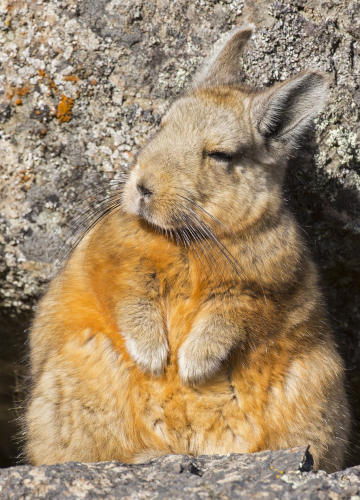
\includegraphics[scale=0.75]{../pictures/viscacha.png} \\
    \end{tabular}
\end{frame}

\subsection{Python}
\begin{frame}
    \frametitle{Python}
    \begin{itemize}
        \item universal high-order programming language
        \item good readability
        \item free
        \item runs on: \\
        \quad \\
        \begin{center}
            \begin{tabular}{ccc}
                
\includegraphics{../pictures/windows_logo.png} \hspace{1cm} &
                
\includegraphics{../pictures/macos_logo.png} \hspace{1cm} &
                
\includegraphics{../pictures/linux_logo.png}
            \end{tabular}
        \end{center}\\
        \quad \\
        \item can be obtained \href{https://www.python.org/}{\textbf{here}}
    \end{itemize}
\end{frame}


\begin{frame}
    \frametitle{Python - Anaconda (recommendation)}
    \begin{columns}
        \begin{column}{.5\textwidth}
            
\includegraphics[scale=0.5]{../pictures/anaconda_logo.png}
        \end{column}
        \begin{column}{.5\textwidth}
            \begin{itemize}
                \item \href{https://www.anaconda.com/products/distribution}{\textbf{Anaconda distribution}} for Windows, MacOS and Linux
                \item Python-centered, but supports also R
                \item easy handling of environments
                \item powerful package manager
                \item latest stable packages
            \end{itemize}
        \end{column}
    \end{columns}
    

\end{frame}


\subsection{ema2wav}
\begin{frame}
    \frametitle{ema2wav}
    \begin{itemize}
        \item converts EMA data into multichannel WAV-files (\& CSVs)
        \item Python-based, only free \& open-source dependencies
        \item supports AG500/501 (Carstens Medizinelektronik GmbH)
        \item multiple options for derivations \& calculations
        \item GUI, command line or python module
        \item work-in-progress
        \item .dmg (MacOS) \& script ($\leftarrow$ always latest version)
        \item can be obtained \href{https://github.com/phbuech/ema2wav}{here}
    \end{itemize}
\end{frame}

\end{document}
